\section{Theorie}
\label{sec:theorie}
In diesem Versuch werden Mikrowellen in Hohlleitern untersucht.

\subsection{Mikrowellen und Hohlleiter}
Als Mikrowellen werden die elektromagnetische Wellen bezeichnet die in einem Frequenzbereich von
1 - $\num{300}\si{\giga\hertz}$ liegen.
Mit
\begin{equation}
  \symup{c} = λ\cdot f
  \label{eqn:geschw}
\end{equation}
folgt der Wellenlängenbereich von 1 - $\SI{300}{\milli\meter}$. \\
Als Hohlleiter werden im Allgemeinen hohle metallische Leiter bezeichnet.
Diese können viele Formen haben wie zum Beispiel rechteckig, oval oder auch
rund.
In diesem Versuch wird ein Rechteckhohlleiter verwendet.
Für Hohlleiter existiert eine minimale Grenzwellenlänge, also die kleinste
Wellenlänge, die sich in einem solchen Leiter ausbreiten kann.
Diese ist definiert als
\begin{equation}
  \lambda_{max} = 2 \cdot b\,.
  \label{eqn:cutoff}
\end{equation}
Dabei ist $b$ die Breite des Hohlleiters.

\subsection{Reflexklystron}
Eine Skizze eines Reflexklystron ist in Abbildung \ref{fig:reflex_klystron} zu sehen.
\begin{figure}[ht]
  \centering
  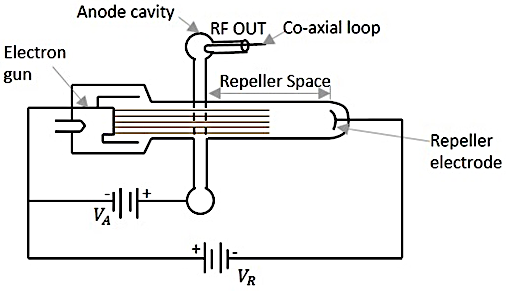
\includegraphics[width=0.8\textwidth]{images/reflex_klystron.png}
  \caption{Skizze eines Reflex-Klystrons \cite{reflex_klystron}}
  \label{fig:reflex_klystron}
\end{figure}
Aus der Elektronenkanone treten durch den Glühelektrischen Effekt Elektronen aus
und werden beschleunigt.
Analog zu einem Kathodenstrahlrohr treffen hier die Elektronen jedoch nicht
auf einen Schirm, sondern werden durch die Reflektorelektrode (rechts) reflektiert.
Dies geschieht aufgrund der Asymmetrie und der in der unteren Kavität anliegenden Spannung so,
dass die Elektronen in die Anodenkavität gelangen.
Hier erzeugen sie durch Influenz ein Elektrisches Feld.
Ein Teil der Elektronen gelangt über diesen Weg in die Kavität,
die anderen werden durch das E-Feld in der Kavität abgelenkt.
Dadurch entsteht ein hochfrequent schwingender Dipol.
Die entstehenden Mikrowellen können durch einen Hohlleiter ausgekoppelt werden.
Durch die mechanische Modifikation des Klystrons kann die Frequenz der austretenen Mikrowellen verändert werden.
\FloatBarrier

\subsection{Stehwellenverhältniss und Methoden}
In einem Hohlleiter bildet sich durch die Überlagerung von hinlaufender und
rücklaufender Welle eine stehende Welle aus.
Durch konstruktive und destruktive Interferenz können im Abstand einer halben Wellenlänge
Knoten und Bäuche entstehen. Dies entspricht dem Idealfall einer stehenden Welle.
Hierfür muss die Beziehung
\begin{align}
  λ_{g,N} &= \frac{2L}{N}
  \intertext{gelten, mit der Hohlleiterlänge $L$ und der Ordnung $N$.
      Im freien Raum gilt}
  λ_0 &= \frac{\symup{c}}{f}\,.
\end{align}

Das Stehwellenverhältnis SWR, welches auch als Welligkeit bezeichnet wird,
beschriebt das Verhältnis der Amplituden von einlaufender und reflektierter Welle.
Es kann Werte zwischen $\infty$ und 1 annehmen.
Falls die Welle nicht reflektiert wird, ist das SWR 1,
da die gesamte Leistung an den Abschluss abgegeben wird.
Wenn am Abschluss ein Kurzschluss eingebaut wird, wird das SWR unendlich, da die
einlaufende Welle vollständig reflektiert wird.
Im Allgemeinen ist das SWR definiert als
\begin{equation}
  \textbf{SWR} = \frac{U_\text{max}}{U_\text{min}} = \frac{\abs{U_\text{Ein}}+\abs{U_\text{ref}}}{\abs{U_\text{Ein}}-\abs{U_\text{ref}}}\,.
\end{equation}

Bei der 3dB Methode werden die Abstände ($\symup{dl}$ und $\symup{dr}$) gemessen, bei der die Leistung
doppelt so groß\, ist wie im Minimum.
Mit dem Zusammenhang
\begin{equation}
  \text{SWR} = \sqrt{\left(1 + \frac{1}{\sin^2\left(\frac{\pi\cdot\left(\symup{dl} - \symup{dr}\right)}{\lambda}\right)}\right)}
  \label{eqn:3dBM}
\end{equation}
kann somit das SWR berechnet werden.

Für die Abschwächer Methode wird herangezogen, dass das SWR berechnet
werden kann, wenn eine Konfiguration von Abschwächungen (D1, D2)
gefunden wird, bei der die Leistung im Minimum gleich der im Maximum ist.
Das bedeutet, nach umstellen von
\begin{align}
  \symup{D2} - \symup{D1} &= 20\cdot \log_{10}(\text{SWR})
  \intertext{nach dem SWR ergibt sich}
  \text{SWR} &= 10^{\left(\frac{D2 - D1}{20}\right)}
  \label{eqn:abschw}
\end{align}

Die Verhältnisse von Amplituden und Leistungen werden in $\si{\deci\bel}$ angegeben.
Es gilt
\begin{align}
  Q &= \log_{10}\left(\frac{P_1}{P_2}\right) \si{\bel} \\
  \SI{1}{\deci\bel} &= \frac{1}{10} \si{\bel}
\end{align}


\subsection{Einwegleitung, Dämpfungsglied und Detektion}
Eine Einwegleitung in einem Hohlleiter wird durch ein Gate realisiert.
Dieses sorgt dafür, dass die gewünschte Laufrichtung der Wellen sehr wenig gedämpft wird,
die unerwünschte nahezu vollständig. Dies kann mithilfe von in den Laufweg der Wellen gekippten Plättchen geschehen.

Dämpfungsglieder für Mikrowellen können unterschiedlich gestaltet sein.
In diesem Versuch wurde eines verwendet, bei dem eine Folie in den Hohlleiter geschoben wird.

Die Detektion von Mikrowellen kann mit Dioden geschehen.
Diese unterscheiden sich dann von Photodioden in der Wahl der Materialien.
%wie bei Lichtwellen über Halbleiterdioden geschehen.
%Es müssen dann nur andere Halbleiter verwendet werden.
